%% Based on <bare_jrnl.tex> in the ieee package available from CTAN,
%% I have changed the options so that most useful ones are clubbed together,
%% Have a look at <bare_jrnl.tex> to understand the function of each package. 

%% This code is offered as-is - no warranty - user assumes all risk.
%% Free to use, distribute and modify.

% *** Authors should verify (and, if needed, correct) their LaTeX system  ***
% *** with the testflow diagnostic prior to trusting their LaTeX platform ***
% *** with production work. IEEE's font choices can trigger bugs that do  ***
% *** not appear when using other class files.                            ***
% Testflow can be obtained at:
% http://www.ctan.org/tex-archive/macros/latex/contrib/supported/IEEEtran/testflow

%        File: icosaeder_description.tex
%     Created: Mon Jul 10 10:00 AM 2006 C
% Last Change: Mon Jul 10 10:00 AM 2006 C
%
\documentclass[12pt, a4paper]{article}
\usepackage{Iem, CustomListings}
\usepackage[english]{babel}
%\usepackage[ansinew]{inputenc}
\usepackage[latin1]{inputenc}
%\usepackage{microtype}
\usepackage{epstopdf}
\usepackage{amsmath, amssymb}
\hyphenation{}
\usepackage{listings}
\usepackage{float}
\usepackage[colorlinks = true,
            linkcolor = black,
            urlcolor  = blue,
            citecolor = blue,
            anchorcolor = blue]{hyperref}
            
\usepackage{url}
%\usepackage{fancyhdr}
%%
%\pagestyle{fancy}
%\renewcommand{\headrulewidth}{0.5pt}

%\fancyhf{}


\usepackage{cite, graphicx, subfigure, amsmath,amssymb} 

% set the graphicspath
\graphicspath{{figures/}} 
\usepackage{placeins, todonotes}

\begin{document}
\selectlanguage{english}
\title{Moody Plant}
\author{Br\"uhwiler Hanna, Elisabeth Hacker, Reiter Michael \\\small{Supervisor: Gro\ss-Vogt, Katharina, Mag.rer.nat. Dr.rer.nat.}}

%\markboth{}{N. Erster, N. Zweiter: Kurztitel}
\markboth{}{Moody Plant}

\doctype{Sonic Interaction Design}

%\date{Juni 2008}

\maketitle
\newpage
\pagestyle{empty}
%\hspace{1cm}\vspace{3cm}

\hspace{1cm}\vspace{1cm}

%\begin{abstract}

\begin{abstract}

This paper documents the creation of the art project 'Moody Plant', an interactive plant that reacts with affectionate sounds to human proximity and touch. Depending on how it is treated, it reacts in three different moods - happy, needy, angry.  The Arduino picks up whether the plant was pet. Via a Pure Data patch, (available on Michael Reiter's  Github\cite{github} the acoustic reactions are determined.
It was created in the course 'Sonic Interaction' by Michael Reiter, Elisabeth Hacker and Hanna Br\"uhwiler and supervised by Katharina Gro\ss-Vogt. 






\end{abstract}



\begin{figure}[H]
\begin{center}
\includegraphics[scale=0.35]{Figures/thumbnail.png}
\end{center}
\end{figure}



\renewcommand{\abstractname}{Kurzfassung}
\begin{abstract}

%Eine Pflanze hat Gef\"uhle. Sie lebt wie jedes andere Lebewesen vor sich hin und wie jeder von uns, braucht sie manchmal etwas N\"ahe und Zuneigung - aber vorsicht, auch nicht zu viel! 'Moody Plant' ist eine interaktive Pflanze, welche im Rahmen eines Gruppenprojekts in Sonic Interaction Design von Michael Reiter, Elisabeth Hacker und Hanna Br\"uhwiler designt und entwickelt wurde. Ihre drei Stimmungen - fr\"ohlich, bed\"urftig, w\"utend - werden \"uber eine Arduino-Verbindung in Pure Data h\"orbar gemacht. Den PD Patch findet man auf Michael Reiters \href{https://github.com/MichaelReiter94/moody_plant}{Github}. 


Diese Arbeit beinhaltet den Entwicklungsprozess des Kunstprojektes 'Moody Plant', eine interaktive Pflanze, die auf menschliche N\"ahe und Ber\"uhrungen reagiert. Sie antwortet akustisch in drei verschiedenen Stimmungen - gl\"ucklich, bed\"urftig und w\"utend. Eine Messvorrichtung mittels Arduino erkennt, wenn die Pflanze gestreichelt wird und schickt diese Daten \"uber eine USB-Verbindung an einen Pure Data Patch. In diesem wird je nachdem wie die 'Moody Plant' behandelt wurde entschieden mit welchen Kl\"angen sie reagieren soll. Der Quellcode dieses Projekts kann auf Michael Reiters Github Seite \cite{github} gefunden werden. 'Moody Plant' wurde im Rahmen des Kurses Sonic Interaction Design von Michael Reiter, Elisabeth Hacker und Hanna Br\"uhwiler entwickelt und wurde hierbei betreut von Katharina Gro\ss-Vogt. 



\end{abstract}

%\end{abstract}
\newpage
\pagestyle{myheadings}
\hspace{1cm}\vspace{2cm}


\tableofcontents
\newpage

% ------------------ MAIN DOC START -----------------------------
\nocite{prosody}
\nocite{couch}
\nocite{plantGrowing}
\nocite{positiveInteraction}
\nocite{github}


\section{Introduction}
A plant has feelings. It lives like every other creature day by day. And like everybody else, it also has some needs. Not only water and sun, but also some affection and physical contact - but careful, not too much! 
This project is a playful attempt to create a more lively communication between humans and plants. The plant is personified, we gave it a voice to be able to interact. It can more be seen as an artistic installation than as a consumer product that serves people to take care of their plants.


\section{Sound Design}


The sound design for the voice of the plant is based on prosody. The plant cannot talk like a human, it communicates its needs through abstract sounds like cats do. It meows, purrs or hisses depending on what mood it is in.


\subsection{Needy Mood}
At the beginning, the plant is quiet and then after a while the needy mood is activated, because it isn't noticed or touched in a while and is kind of in need of attention. The sounds for that particular mood are whiny (going down with the voice), questioning (going up with the voice), weeping (like a baby or a cat). The intention behind that sound decision is the human consciousness of that noises and by hearing them they recognize that something is wrong, the plant is unhappy and is in need of something.  

In total, we created 13 sounds for this mood which you can hear on Github \cite{github} mentioned in the abstract. 



\subsection{Happy Mood}
The happy mood starts as soon as the plant gets attention from the people around her. It reacts on people who are close or touch the leaves of the plant. But it only stays in the happy mood as long as it is not overwhelmed with attention. While the plant sounds happy, the people hear sounds of relief, carefree and satisfied. This is mapped with the sounds of for example a happy cat purring  or as mentioned earlier a happy baby. 

For this particular mood, we created 14 short sound snippets which you can find on  Github \cite{github}.



\subsection{Angry Mood}

By giving the plant too much attention, the happy mood changes into the angry mood where the plant rejects the fondling of the people. The noises it makes in that mood are hissing, high barking and  fast and short sound phrases. This should signal the people that the  plant wants to be left alone and needs space. 
After a while with no attention, the plant starts to get needy again and switches to the first mode.

The angry mood has a variety of 12 different sounds which are chosen randomly through the patch which you can all find on  Github \cite{github}.

\section{Technical Implementation}
In order to be able to trigger a sonic reaction by the plant by touching it, a reliable sensor with appropriate signal processing needs to be implemented. In this case we chose to measure the capacitance in a way. These changes are picked up by an Arduino, which transfers the data via USB port to a computer. The data is received within a Pure Data patch which decides when to play what kind of samples. In a later attempt we tried a standalone variant with a Raspberry Pi instead of a computer.

\subsection{Measuring Capacitance}
For the capacitance measurement we send a 100 Hz square wave signal through a digital output. This means the binary output switches between 0 and 5 Volts. The signal goes thorugh a $10 M \Omega$ resistor and then into the soil of the plant. The analogue input of the Arduino measures the voltage between the resistor and its internal ground. Since the plant soil is not connected in any way to the internal ground, the voltage between is not defined. A difference in voltage when the resistance changes can be detected nevertheless. 

\begin{figure}[H]
\begin{center}
\includegraphics[width=0.7\linewidth]{Figures/schematic1.png}
\caption{Schematic of the measuring set-up}
\end{center}
\end{figure}
Since with this set-up, the measurements change drastically with the environment and used equipment (PC, Raspberry Pi,...) a calibration method was implemented in Pure Data to adjust for the changes.


\subsection{Processing Input Data}
\subsubsection{Arduino}
Once the input data is received, it needs to be filtered. First a DC-Filter is applied since we do not want any DC offsets but also because we do not care for low-frequency content when analysing capacitance. Next, a Root Mean Square value is calculated to smooth out the received data. The input pin is read with a sampling frequency of 800 Hz and every $25^{th}$ sample, a RMS over 1024 samples is sent to the serial output with a alphabetical prefix. Numerical values go from 0 to 1023, the alphabetical prefix determines the sensor (a light sensor or a moistness sensor might be implemented at a later time) so they can be told apart after transmission. 
\subsubsection{Pure Data}
Once the data is received in Pd, it first needs to be converted from ASCII to numbers, so that the algorithm can further process the information:

%\begin{figure}[H]
%\begin{center}
%\includegraphics[width=0.7\linewidth]{Figures/ASCII.png}
%\caption{Converting ASCII data received from the Arduino to integers}
%\end{center}
%\end{figure}
Afterwards, the kind of reaction (happy, needy or angry) needs to be determined. For this, the program needs to know when a touch occurs. This is achieved by the calibration process. By touching the plant, standing close to it and going away from it during calibration, it sets the thresholds for when it is supposed to detect a touch or proximity.
\begin{itemize}
\item Happy:\\
If the input goes beneath the set threshold, it plays a happy sound (randomly chosen but non repeating). Afterwards the Pd patch ignores all touches for a certain amount of time (as of now 700 miliseconds) before being able to play any sound again. This is necessary because we get about 30 values per second that would trigger 30 sounds within this second if the plant was touched for this entire second.
\item Angry\\
If, within a set amount of time the plant was touched too much, it expresses anger. The amount of time until it becomes annoyed can be set in the GUI. So if, for example, you have been touching it for four seconds within the last ten seconds everything is fine. If you have been holding its leaves for five or more seconds in that time it gets angry.
\item Needy\\
As soon as you let go of the plant, a timer starts counting. If the timer reaches a threshold set in the GUI, the plant becomes needy. This does not mean it constantly makes noises for attention but every second there is a small probability for it to make a noise. If in this state you get in close proximity to the plant (not touching it, just passing by next to it), it will very likely call you out and demand some love.
\end{itemize}

\begin{figure}[H]
\begin{center}
\includegraphics[width=0.9\linewidth]{Figures/calculateTouches.png}
\caption{Calculating if it has been touched, touched for too long or not had any attention for too long}
\end{center}
\end{figure}

\begin{figure}[H]
\begin{center}
\includegraphics[width=0.9\linewidth]{Figures/decideMood.png}
\caption{Decide on what mood to express}
\end{center}
\end{figure}
\subsubsection{Graphical User Interface}
The GUI in Pd has consists of three parts: Calibration, monitoring and settings.


\begin{figure}[H]
\begin{center}
\includegraphics[width=0.9\linewidth]{Figures/GUI.png}
\caption{Graphical User Interface}
\end{center}
\end{figure}


The calibration in the top part has already been described. It sets the correct threshold. Just push the 'start calibration button' and the text field tells you what to do when.
The middle part is mostly for settings like which USB port to read from, opening and closing the port and setting the time for when mood changes occur and what sound character to use (so far we have recorded two different kinds of characters with happy, angry and needy sounds each). Lastly the incoming voltages can be monitored. On the very bottom, two graphical arrays are displayed. If a plant is connected, they show the history of the last 100 samples. The only difference between them is the y-scaling. One is zoomed further in for the proximity detection (visibly only as smaller changes) and one adjusted to the 'touch-threshold'. The buttons on the right display if the algorithm detects a touch, proximity or nothing at all at this very moment. 





\subsection{Standalone Version}
As an additional task, we tried to get the entire system running without needing to connect it to a computer. One reason for this attempt was, that we wanted the project to be a part of an exhibition. Instead of a computer, a Raspberry Pi was used on which Pure Data was installed. Unfortunately the Pd object for reading the serial input did not work. As a workaround a python script was written which reads the serial input and sends the data via OSC, which in turn can be read by Pure Data:
\begin{lstlisting}[style=styC++]
import time
import serial
from pythonosc import udp_client

ser = serial.Serial('/dev/ttyACM0', 9600, timeout=5)
client = udp_client.SimpleUDPClient("127.0.0.1", 8000)
while 1:
    input_string = ser.readline().decode("utf-8").strip()
    print(input_string)
    client.send_message("/A", int(input_string[1:]))
    time.sleep(0.001)
\end{lstlisting}
This script has to be running constantly for the Pd patch to work. If an error occurs (e.g. by unplugging the USB connection shortly), the script may stop and everything will stop working. Additionally, the USB port is set in the script and if the Arduino is plugged in another port it will not work either unless you change the code.
\begin{figure}[H]
\begin{center}
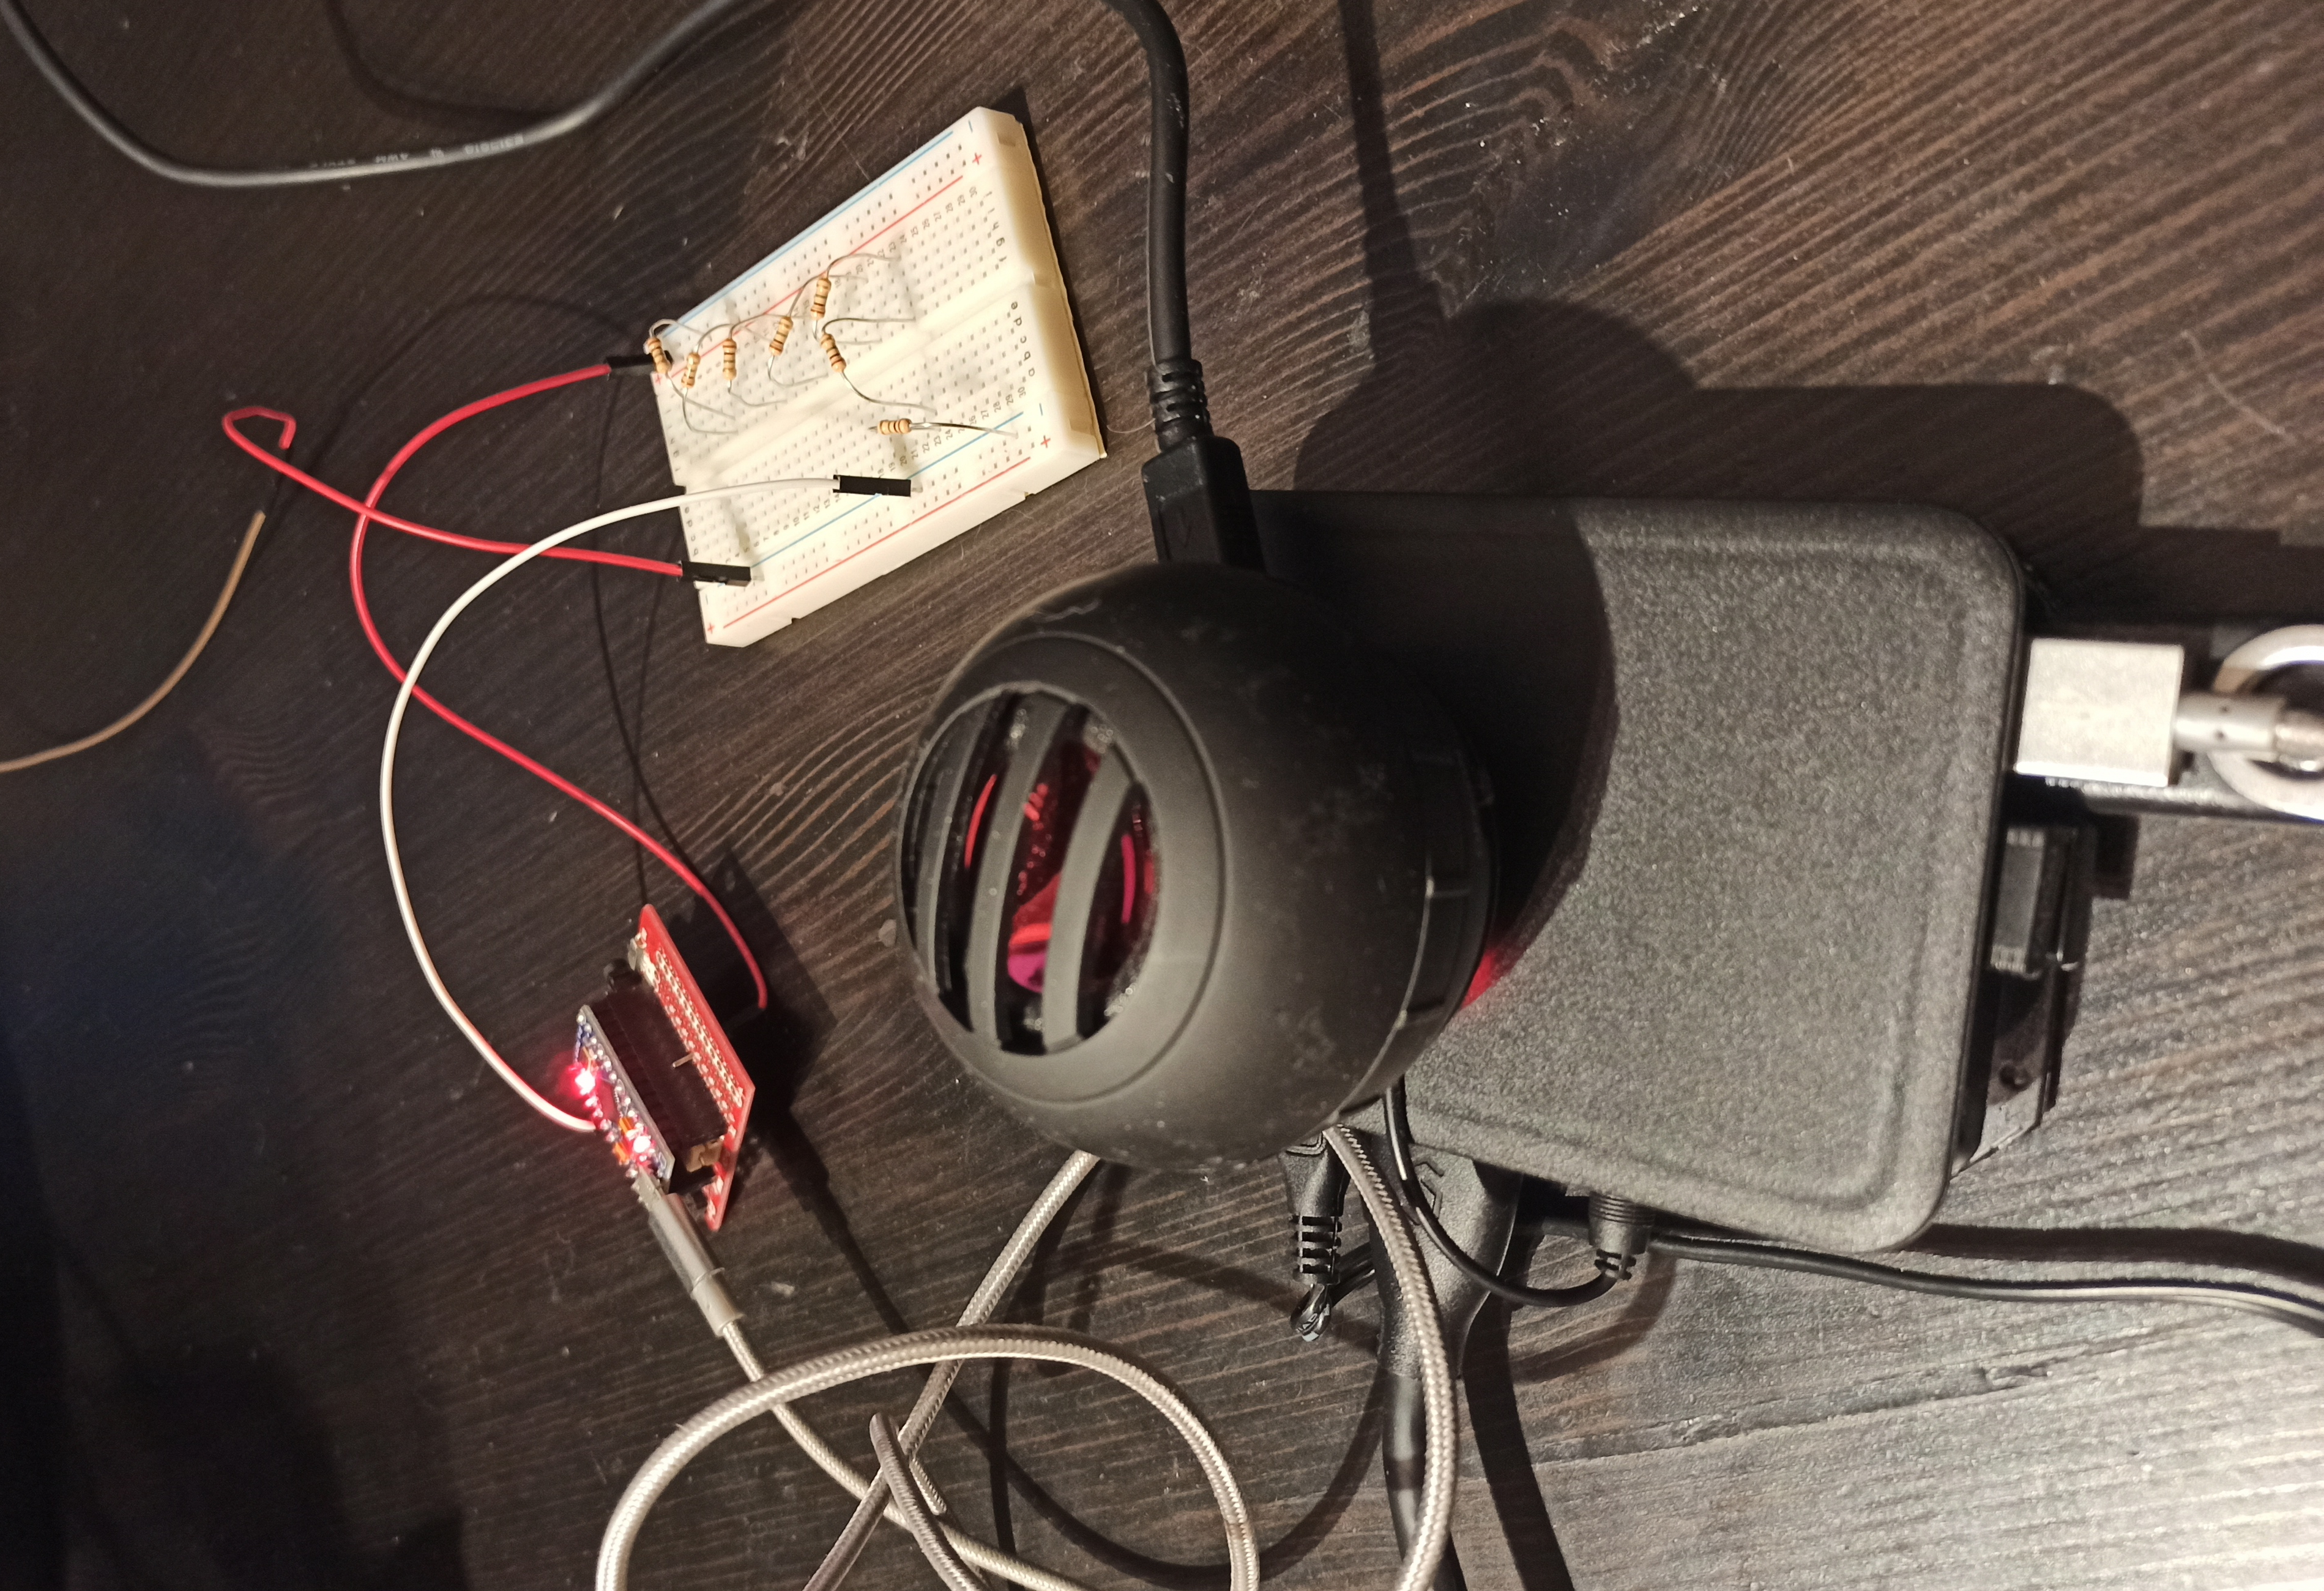
\includegraphics[width=0.75\linewidth]{Figures/setup.jpg}
\caption{Arduino, Raspberry Pi and battery powered speaker}
\end{center}
\end{figure}









\section{Presentation}

For the demonstration of our project, we created a short video to show what our sonic art installation 'Moody Plant' actually does and how it works. You can see our video documentation on Youtube \cite{youtubeDemo}.

The plant was issued in the exhibition 'Union Reflection Assembly' by the degree program Communication, Sound and Interaction Design at FH JOANNEUM in Graz. It got its main performance during the livestream of the vernissage on 27th february 2021, where it communicated with the moderators and even made it to Austrias public broadcasting ORF. For its big show we gave it the name 'Annabelle LaNoir'.


\begin{figure}[H]
\begin{center}
\includegraphics[width=0.8\linewidth]{Figures/plant2.jpg}
\caption{Moody Plant 'Annabelle LaNoire' dressed up for the big show}
\end{center}
\end{figure}



If you are interested, you can watch the live stream \cite{liveStream} at 54:54. 


\section{Conclusion and Outlook}

Reflecting on the project, it was a fun project working together with Annabelle LaNoire. It must be said that it should only be seen as an art installation and not as an auditive reminder of what the plant actually needs.  So the purpose of our project 'Moody Plant' was more the interaction with and personalization of the plant in a gamified way. It was also intended to raise the awareness of the user to the fact that the plant is a slow, yet living creature comparable in some ways to pets. 
This goal was achieved and by including it into the URA Reflection Assembly Exhibition of the CMS19 master study. It reached a wide range of people and was a 'ear catcher' at the preparation of the exhibition, although Annabelle was a bit shy at the actual live streaming event. 

As an outlook, we could create two kinds of consumer products from this concept: \\
On the one hand, we could change the mapping of the sound design to have a more useful aspect for the plant itself. So that the plant not only makes sounds caused by the physical interaction with people, but that it instead makes heard of its need for water, light, a bigger pot or fresh potting soil. So the sound design concept could be used for plant sensors that communicate in a more practical way with the users.   \\
On the other hand, the optimization of the technical implementation is kept in mind. By 3D printing a plant pot with the opportunity to add a loudspeaker, the needed technical equipment and an easier way to calibrate the settings, a more consumer friendly product would be created. After the optimization, the only thing a user has to buy is the 'Sonic Plant Pot' to make their own house plant a moody plant. Additional improvements could be self-adjusting thresholds that adept to a change in surroundings to make calibration obsolete. Another possible change would be to have a power supply without needing to plug it in with a cable. It could either be solved by using batteries or maybe even with photovoltaic panels. Finally it would make sense to use only one of our devices, be it the Arduino or the Raspberry Pi.











% ------------------
% ------------------ MAIN DOC END -----------------------------
\newpage
\bibliography{BibDatabase}
\bibliographystyle{ieeetr}

\end{document}